\chapter{Diseño de sistema}
Este capítulo presenta los requerimientos específicos de software que definen las funcionalidades y 
restricciones. Con base a ello, se desarrolla el diseño conceptual, modular y detallado del sistema, 
así como la definición de la arquitectura de datos, software y nube que sustenta su implementación.
\section{Requerimientos específicos de software}
\textbf{Explicación de nomenclatura.}
\begin{itemize}
    \setlength{\itemsep}{0pt}
    \setlength{\parskip}{0pt}
    \setlength{\parsep}{0pt}
    \setlength{\topsep}{0pt}
    \item RF: Requisito funcional.
    \item RNF: Requisito no funcional. 
    \item RI: Requisito de interfaz.
    \item RIM: Requisito de implementación.
\end{itemize}

\begin{table}[H]
\centering
\small
\renewcommand{\arraystretch}{1.2}
\caption{Requerimientos de implementación}
\label{tab:req_imp}
\begin{tabularx}{\textwidth}{%
    >{\raggedright\arraybackslash}p{0.08\textwidth}
    >{\raggedright\arraybackslash}p{0.08\textwidth}
    >{\raggedright\arraybackslash}p{0.23\textwidth}
    >{\raggedright\arraybackslash}X
}
\toprule
\textbf{Tipo} & \textbf{ID} & \textbf{Título} & \textbf{Descripción} \\
\midrule
RIM & A & Arquitectura de software &
La implementación de todos los módulos debe seguir una arquitectura basada en microservicios con un patrón de diseño orientado a eventos. \\
RIM & B & Acceso a código &
El código debe subirse a GitHub con una estructura monorepositorio que separe el frontend, la base de datos y el backend. \\
RIM & C & Tecnologías de frontend &
La plataforma web debe construirse con Vue.js y Nuxt para la comunicación con el backend, utilizando módulos de TypeScript. \\
RIM & D & Tecnologías de base de datos &
La base de datos debe construirse con PostgreSQL y pgvector, respetando el diseño de arquitectura entidad-relación. \\
RIM & E & Tecnología de orquestación &
La orquestación de eventos debe construirse con Redis. \\
RIM & F & Tecnología de backend y API REST &
La API debe construirse con FastAPI y Python, mientras que los microservicios deben utilizar modelos Pydantic e implementarse con Python. \\
RIM & G & Integración CI/CD &
La integración y el despliegue continuos deben implementarse mediante GitHub Actions. \\
RIM & H & Tecnologías de nube &
El despliegue del servicio debe realizarse mediante la plataforma Google Cloud. \\
\bottomrule
\end{tabularx}
\end{table}

\begin{table}[H]
\centering
\small
\renewcommand{\arraystretch}{1.15}
\caption{Requerimientos generales de interfaz}
\label{tab:req_int}
\begin{tabularx}{\textwidth}{%
    >{\raggedright\arraybackslash}p{0.08\textwidth}
    >{\raggedright\arraybackslash}p{0.08\textwidth}
    >{\raggedright\arraybackslash}p{0.23\textwidth}
    >{\raggedright\arraybackslash}X
}
\toprule
\textbf{Tipo} & \textbf{ID} & \textbf{Título} & \textbf{Descripción} \\
\midrule
RI & I & Tipografía principal &
Se establece IBM Plex Sans como la única familia tipográfica sans-serif para toda la interfaz. \\
RI & J & Jerarquía tipográfica y tamaños &
\begin{itemize}[leftmargin=*,nosep]
    \item Cuerpo base de texto: 18 px.
    \item Títulos principales (H1): 32 px.
    \item Títulos secundarios (H2): 24 px.
    \item Texto secundario y metadatos: 16 px.
\end{itemize} \\
RI & K & Interlineado y espaciado &
\begin{itemize}[leftmargin=*,nosep]
    \item Interlineado general: 1.5.
    \item Interlineado para campos abiertos: 1.6.
    \item Espaciado para títulos: 0.01 em.
    \item Margen inferior de bloques: 1.25 rem.
\end{itemize} \\
RI & L & Paleta de colores &
\begin{itemize}[leftmargin=*,nosep]
    \item Fondo general: \#A8C1B6.
    \item Texto principal: \#2E2E2E.
    \item Elementos interactivos: \#53C9AF.
    \item Mensajes de error: \#DB3539.
\end{itemize} \\
RI & M & Arquitectura de navegación &
La navegación debe presentar una estructura secuencial fragmentada en pantallas. \\
RI & N & Indicador de progreso &
La interfaz debe mostrar un indicador minimalista que marque el avance actual. \\
RI & O & Microinteracciones y animaciones &
Las transiciones de pantalla y animaciones de botones deben reducirse al mínimo. \\
RI & P & Estilo de UI/UX &
La plataforma deberá utilizar un estilo denominado glassmorfismo. \\
RI & Q & Representación de métricas &
Los resultados deberán visualizarse mediante gráficos y una explicación textual de los datos de coincidencia. \\
\bottomrule
\end{tabularx}
\end{table}

\begingroup
\small
\renewcommand{\arraystretch}{1.15}
\begin{xltabular}{\textwidth}{%
    >{\raggedright\arraybackslash}p{0.08\textwidth}
    >{\raggedright\arraybackslash}p{0.10\textwidth}
    >{\raggedright\arraybackslash}p{0.23\textwidth}
    >{\raggedright\arraybackslash}X
}
\caption{Requerimientos generales}
\label{tab:req_gen} \\
\toprule
\textbf{Tipo} & \textbf{ID} & \textbf{Título} & \textbf{Descripción} \\
\midrule
\endfirsthead
\multicolumn{4}{c}{\tablename\ \thetable{} -- Continuación} \\
\toprule
\textbf{Tipo} & \textbf{ID} & \textbf{Título} & \textbf{Descripción} \\
\midrule
\endhead
\bottomrule
\endfoot
\bottomrule
\endlastfoot

RF & 1 & Información en pantalla de inicio &
La plataforma deberá presentar información introductoria sobre el sistema, su objetivo, su funcionamiento y la forma adecuada de responder el cuestionario. El botón ``Comenzar'' deberá dirigir a la pantalla de recopilación de datos personales. \\

RI & 1.1 & Pantalla de inicio &
La pantalla deberá incluir la frase ``Descubre tu camino profesional'', un texto introductorio, una explicación del funcionamiento y un botón ``COMENZAR'', en un orden claro y centrado. \\

RF & 2 & Cuestionario de información personal &
La plataforma deberá mostrar campos para capturar el nombre y el correo electrónico, además de un botón ``Siguiente''. \\

RNF & 2.1 & Restricciones del campo de nombre &
El campo ``Nombre'' deberá admitir únicamente caracteres alfabéticos y una longitud de 3 a 60 caracteres. \\

RNF & 2.2 & Restricciones del campo de correo electrónico &
El campo deberá aceptar únicamente direcciones con formato válido, compuesto por usuario, símbolo ``@'' y dominio. \\

RNF & 2.3 & Uso de datos personales &
Los datos recopilados se utilizarán exclusivamente con fines estadísticos. Proporcionarlos no constituirá un registro ni creará una cuenta. \\

RF & 2.4 & Términos y condiciones &
La plataforma deberá mostrar una casilla de aceptación, desmarcada por defecto, y un enlace para consultar los términos. La aceptación será obligatoria para continuar. \\

RI & 2.5 & Pantalla de cuestionario de información personal &
La pantalla deberá mostrar los campos de nombre y correo electrónico, el aviso sobre el uso de datos, el acceso a los términos, la casilla de aceptación y el botón ``Siguiente''. Los elementos deberán ser legibles, ordenados y adaptables. \\

RF & 3 & Cuestionario de selección de área &
La plataforma deberá permitir seleccionar una sola área de conocimiento y mostrar el cuestionario correspondiente. \\

RNF & 3.1 & Selección de área &
La selección deberá limitarse a Ingeniería y Ciencias Físico-Matemáticas, Ciencias Médico-Biológicas o Ciencias Sociales y Administrativas. No se permitirán áreas manuales o distintas. \\

RI & 3.2 & Pantalla de selección de área &
La pantalla deberá presentar el título ``Selecciona tu área de conocimiento'', el texto de apoyo y tres tarjetas uniformes con indicador de selección, ícono y nombre del área. \\

RF & 4 & Cuestionario de selección de habilidades &
La plataforma deberá mostrar la pregunta sobre las fortalezas de la persona usuaria, permitir múltiples selecciones y avanzar mediante el botón ``Siguiente''. \\

RNF & 4.1 & Catálogo de habilidades &
El catálogo deberá integrar las habilidades de los perfiles de ingreso de las carreras del IPN y mostrar únicamente las correspondientes al área seleccionada. \\

RNF & 4.2 & Selección de habilidades &
La persona usuaria deberá seleccionar al menos una habilidad para continuar. \\

RI & 4.3 & Pantalla de selección de habilidades &
La pantalla deberá mostrar la pregunta, una lista vertical de habilidades con casillas de selección y un botón ``Siguiente'', manteniendo contraste y legibilidad. \\

RF & 5 & Cuestionario STAR &
La plataforma deberá presentar cuatro situaciones para identificar habilidades a partir de experiencias previas. Cada respuesta deberá organizarse en situación, tarea, acción y resultado. \\

RNF & 5.1 & Restricciones de entradas de texto en cuestionario STAR &
Las respuestas deberán ser claras, detalladas y relacionadas con la pregunta. Las respuestas insuficientes deberán notificarse sin interpretarlas como ausencia de habilidades. \\

RI & 5.2 & Pantallas de cuestionarios STAR &
Las preguntas deberán mostrarse con tipografía legible y cuadros de texto de varias líneas, manteniendo un estilo uniforme. \\

RF & 6 & Resultados &
La plataforma deberá mostrar las tres carreras con mayor porcentaje de coincidencia, ordenadas de mayor a menor, junto con sus escuelas y un botón para descargar el reporte. \\

RNF & 6.1 & Interacción con resultados &
Cuando ninguna carrera alcance el porcentaje mínimo, deberá mostrarse una pantalla de ausencia de resultados con las opciones ``Intentar nuevamente'' y ``Elegir otra área''. \\

RF & 6.2 & Pantalla de error &
Cuando no exista una coincidencia suficiente, la plataforma deberá informar que no fue posible generar una recomendación y permitir intentarlo nuevamente o elegir otra área. \\

RI & 6.3 & Pantalla de resultados &
La pantalla deberá mostrar el título de resultados, las carreras recomendadas, el porcentaje de coincidencia, las escuelas y el botón ``Descargar reporte'', con un diseño visual consistente. \\

RI & 6.4 & Pantalla de error en resultados &
La pantalla deberá mostrar un mensaje informativo sobre la coincidencia insuficiente y los botones ``Intentar nuevamente'' y ``Elegir otra área''. \\

\end{xltabular}
\endgroup



\section{Diseño conceptual}
\begin{figure}[H]
\centering
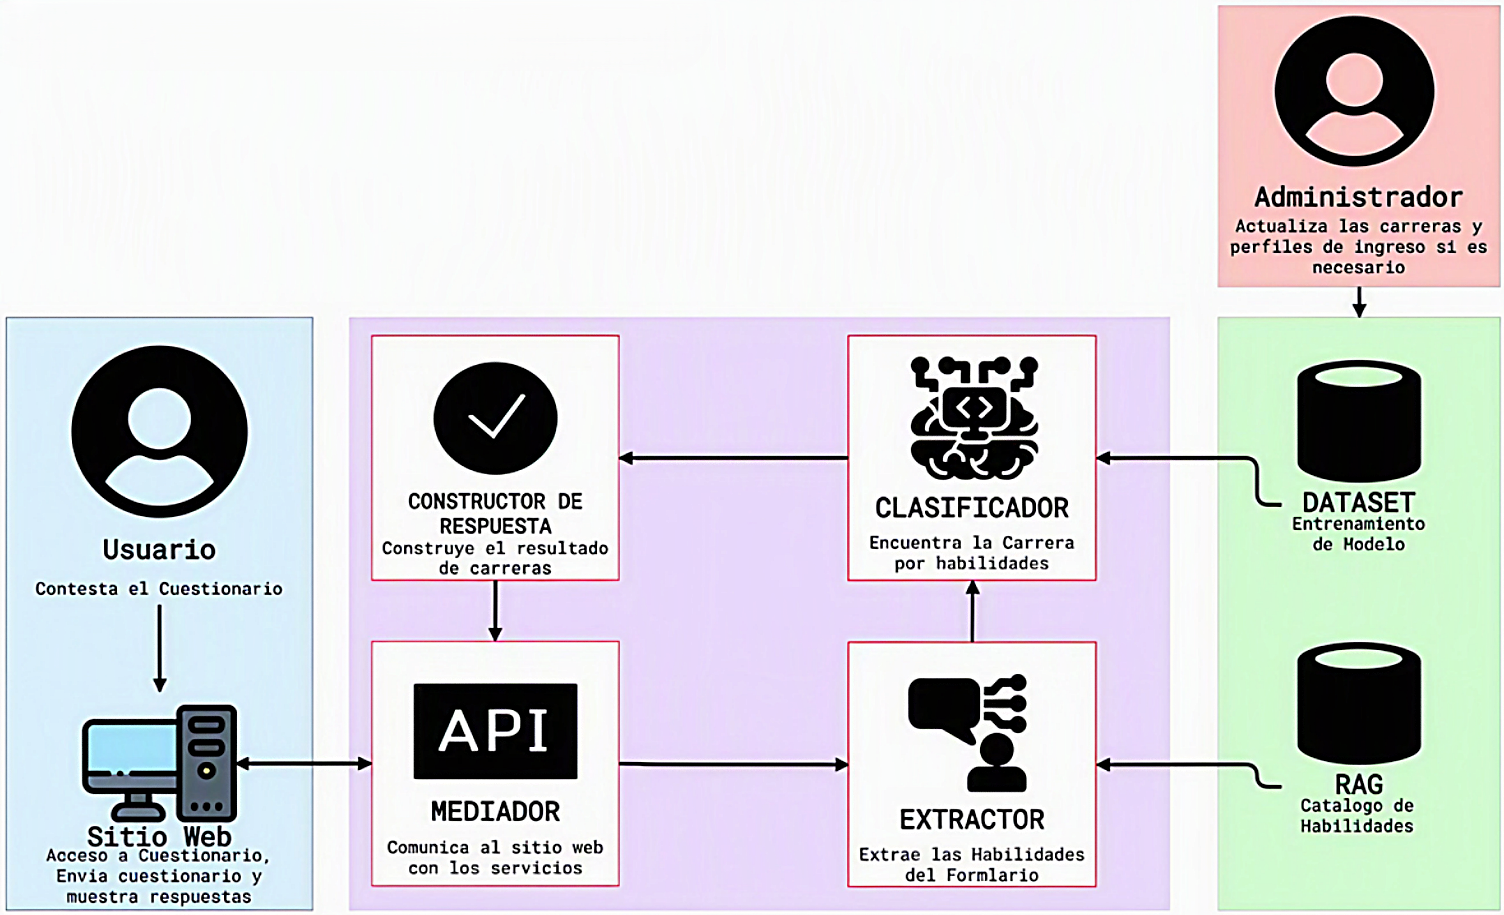
\includegraphics[width=\textwidth]{imagenes/dConceptual.png}
\caption{Diseño conceptual del sistema}
\label{fig:diseno-conceptual}
\end{figure}

\section{Diseño modular}
\begin{figure}[H]
\centering
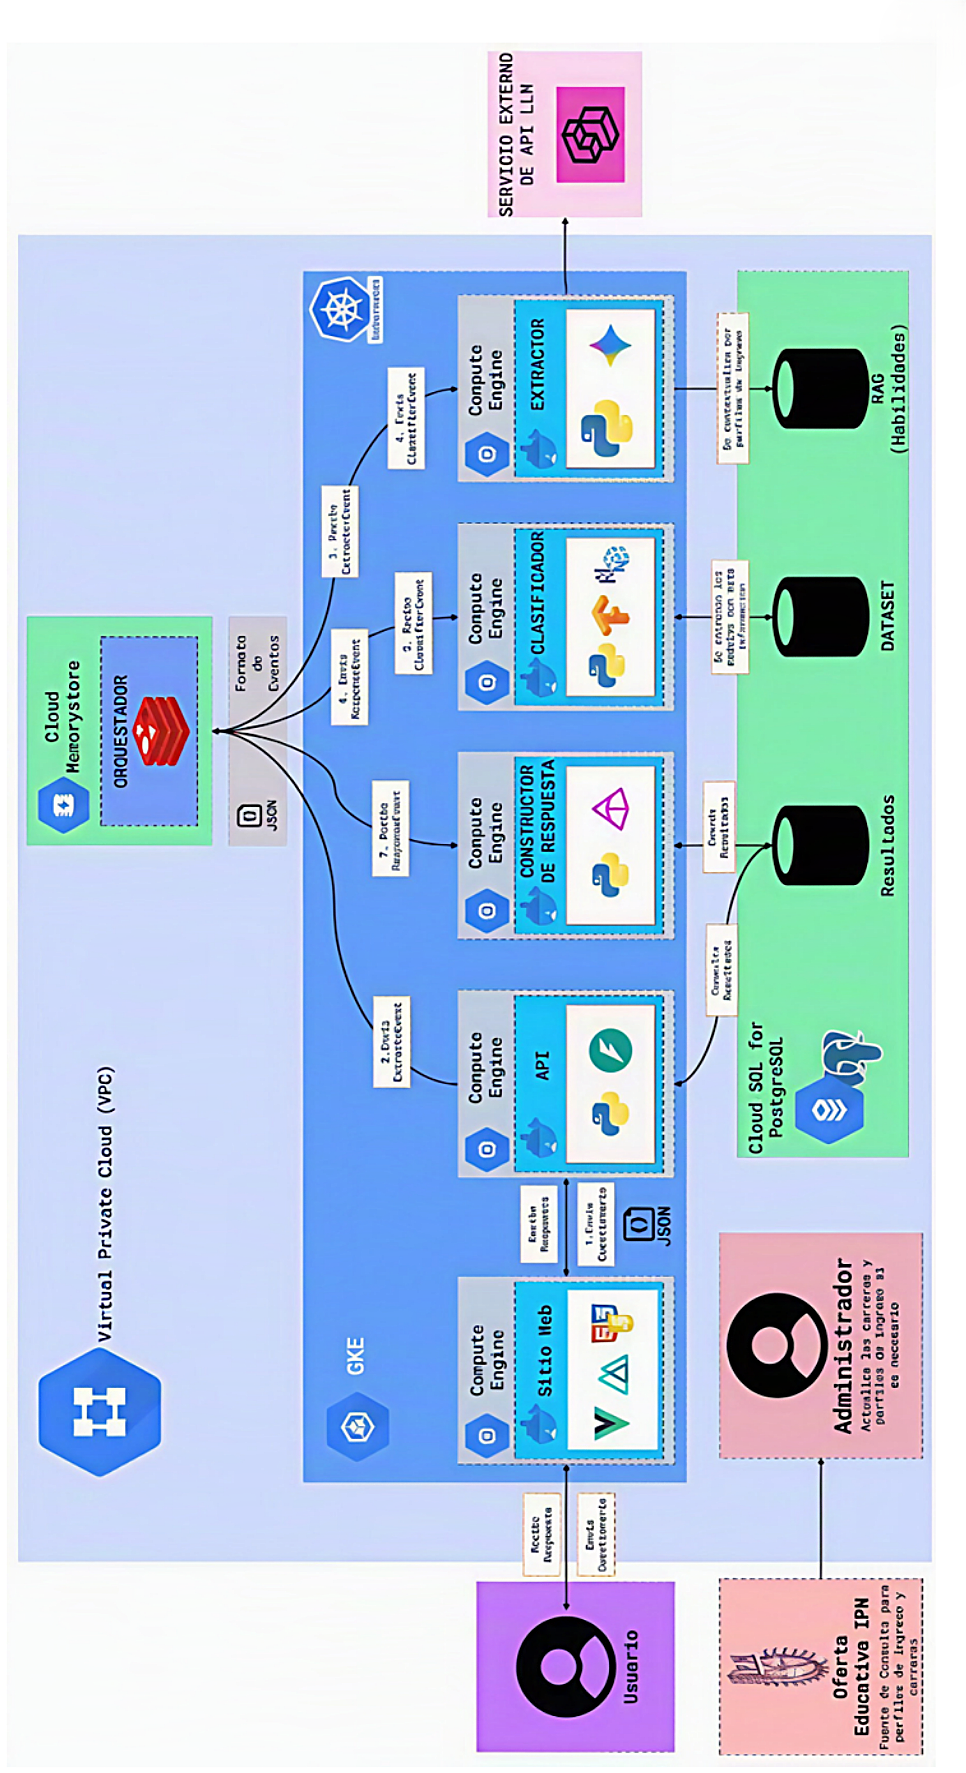
\includegraphics[height=0.81\textheight,keepaspectratio]{imagenes/dModular.png}
\caption{Diseño modular del sistema}
\label{fig:diseno-modular}
\end{figure}

\section{Diseño detallado}
\subsection{Arquitectura de base de datos}
\begin{figure}[H]
\centering
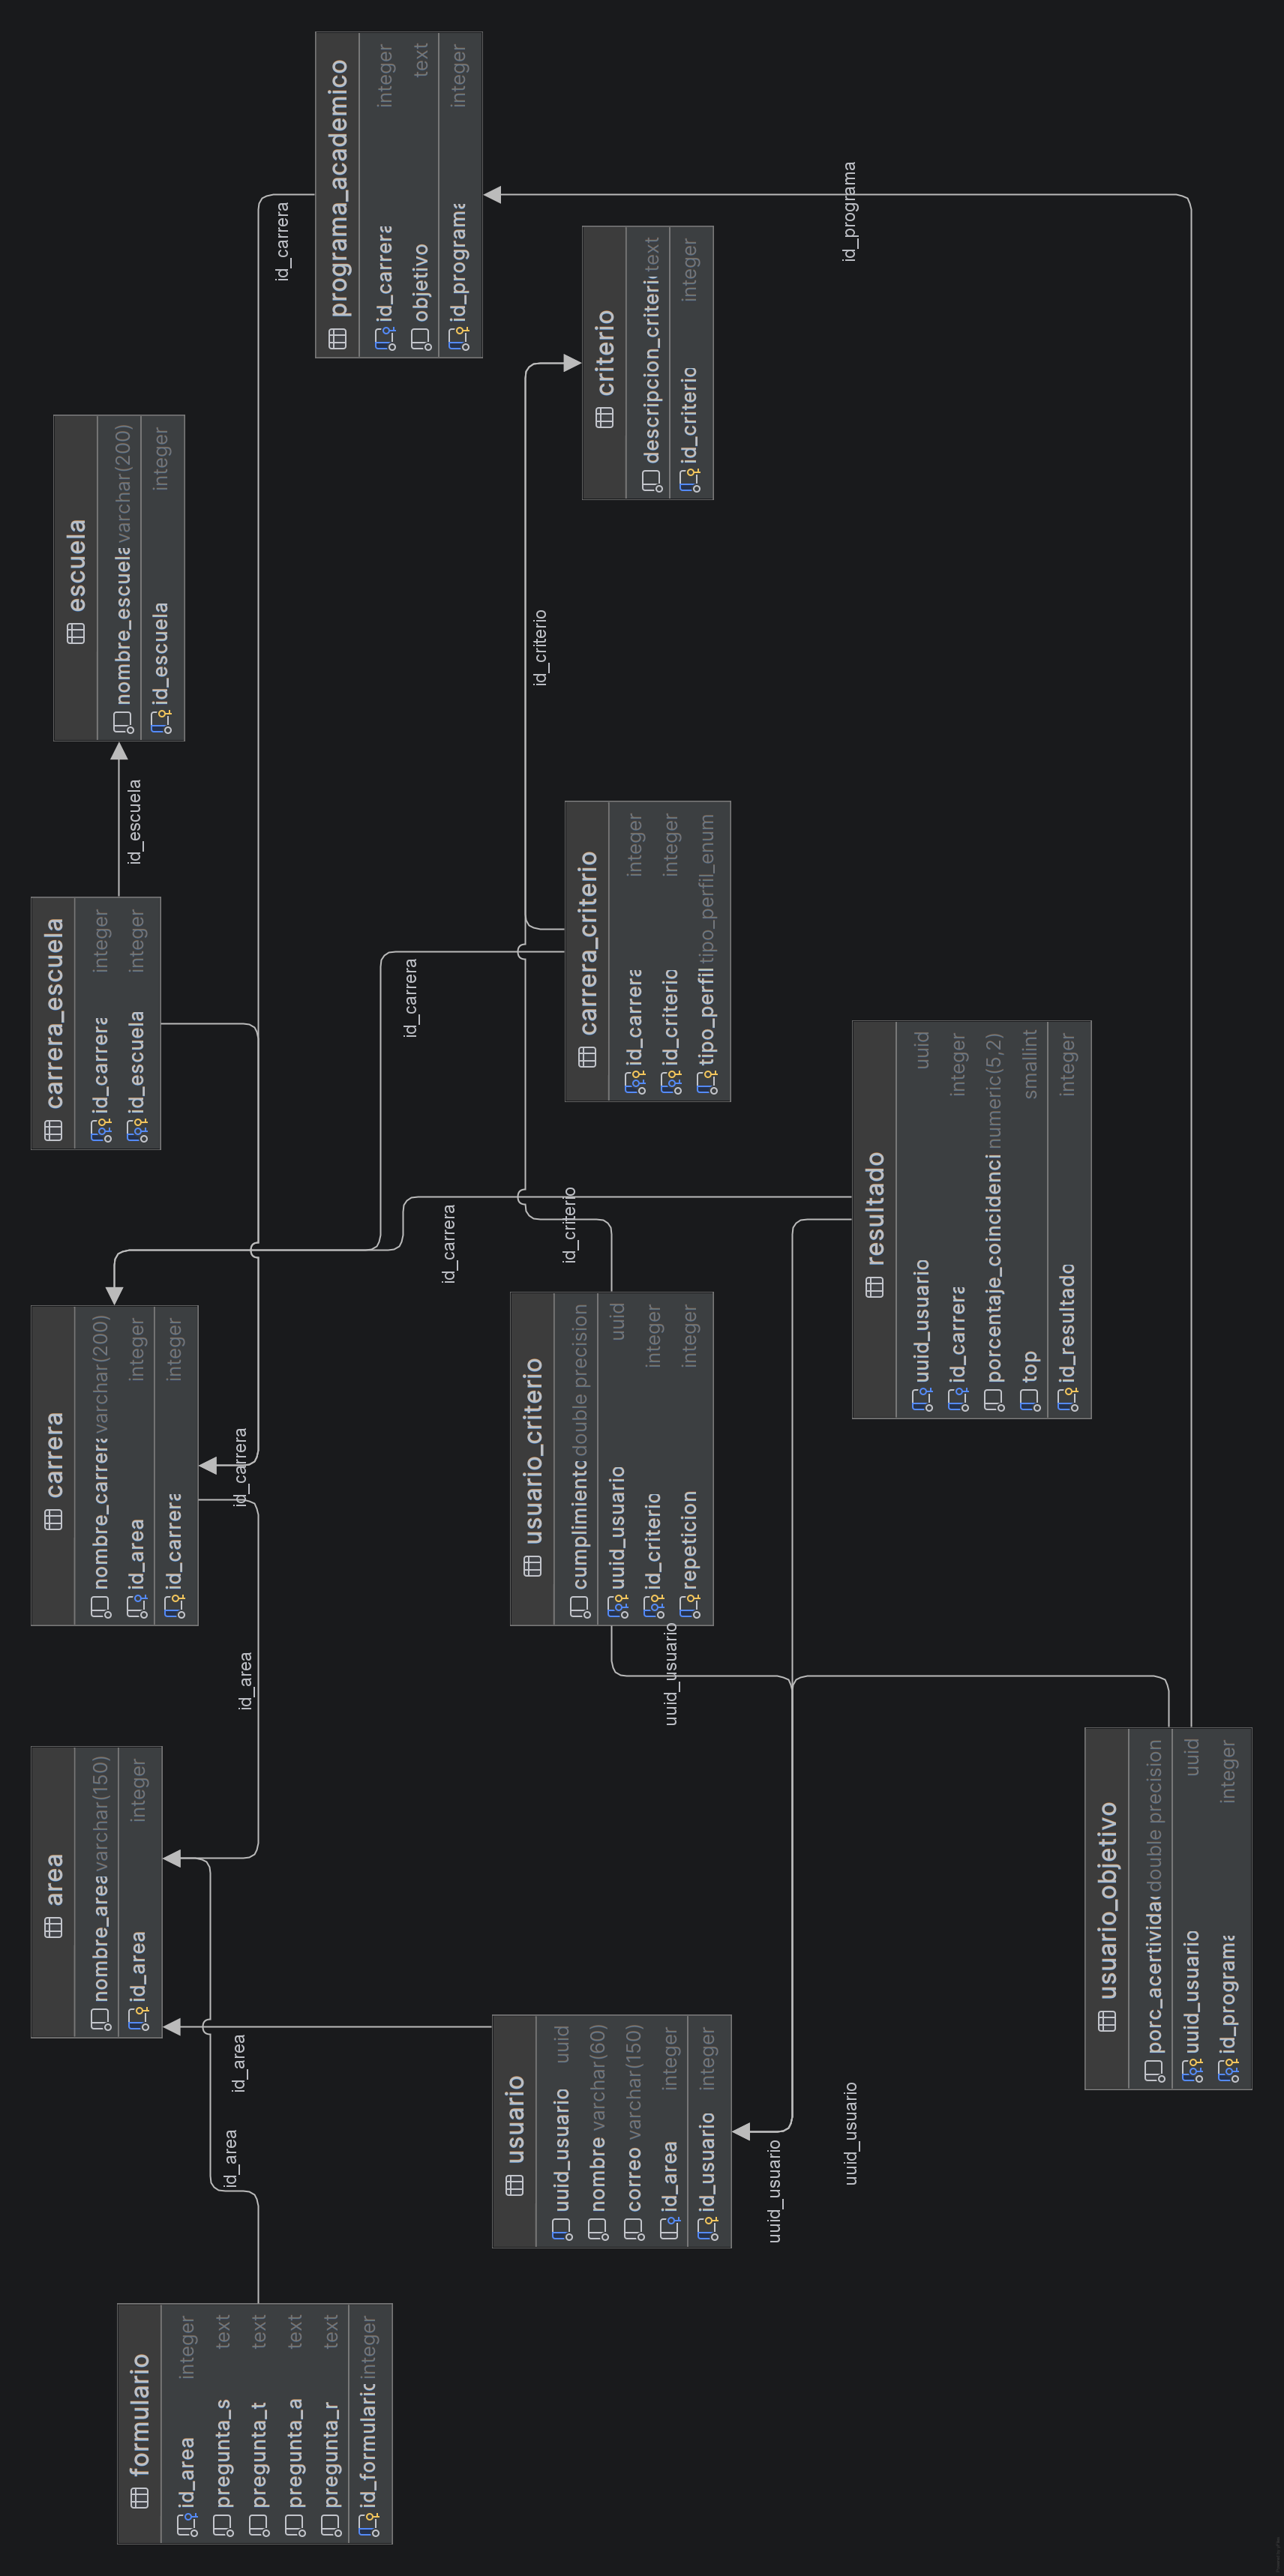
\includegraphics[height=0.81\textheight,keepaspectratio]{imagenes/athenaBD.png}
\caption{Arquitectura de la base de datos Athena}
\label{fig:arquitectura-base-datos}
\end{figure}

\subsection{Diagramas de flujo modulares}
\subsection{Arquitectura de software}
\subsection{Arquitectura de nube}
%%%%%%fin del archivo
\endinput 